

\subsection{Принципиальная схема устройства исполнительного управления }

Принципиальная схема устройства исполнительного управления мини робота манипулятора представлена на рисунке \ref{PACD}. Микроконтроллер U9 является главным вычислительным компонентом исполнительной системы управления. Чип STM32G431CBU6 подключен по стандартной схеме, из даташита \citep{STM32G431}DC-DC преобразователь является главным источником питания для всего устройства исполнительного управления, а микроконтроллер работает с аналоговым сигналом. Для повышения стабильности работы аналоговых операционных усилителей и точности работы АЦП  в схеме реализован фильтр подавления шумов на линии аналогового питания VDDA и линии опорного напряжения VREF+, который собран по заметкам AN5346 (STM, 2019). Микроконтроллер тактируется при помощи кварцевого резонатора X1 и X2, которые подключены по стандартной схеме с конденсаторами C23, C24 для X1 и С18,С19 для кварцевого резонатора X2. Кварцевый резонатор X1 является  главным генератором тактирующего HSE сигнала 8 МГц для микроконтроллера U9. Кварцевый резонатор X2 имеет специфичную  низкоскоростную частоту LSE 32.768kHz, резонатор необходим для работы часов реального времени RTC, часы используются для точного отсчета времени без накопления ошибки в случае двоичного преобразования. Для программирования микроконтроллера выводы программатора-отладчика выведены на разъём H2.

Для контроля состояния исполнительного устройства предусмотрены два светодиода LED1 и LED2. Светодиод LED1 подключен через токовый резистор к питанию и загорается при поступлении питания, LED2 загорается при необходимости от сигнала МК и является индикатором ошибки работы исполняющего устройства.  К входу АЦП PA0 микроконтроллера подключен делитель входного напряжения, состоящий из резисторов R16 и R18, номиналы сопротивления выбраны более 10 kOhm для предотвращения большого падения напряжения на резисторах, максимальное возможное измеряемое напряжение 33 Вольта. Второй вход АЦП PB14 подключен к выводам схемы измерения температуры, которая состоит из NTC резистора R15 и балансного сопротивления R20,конденсатор C30 является элементом фильтра низкой чистоты, верхняя граничная частота  1.5 kHz.

\begin{figure}[H]
	\begin{adjustbox}{addcode={\begin{minipage}{\width}}{\caption{
							Принципиальная схема системы исполнительного управления
						} \label{PACD}
					\end{minipage}},rotate=90,center}
		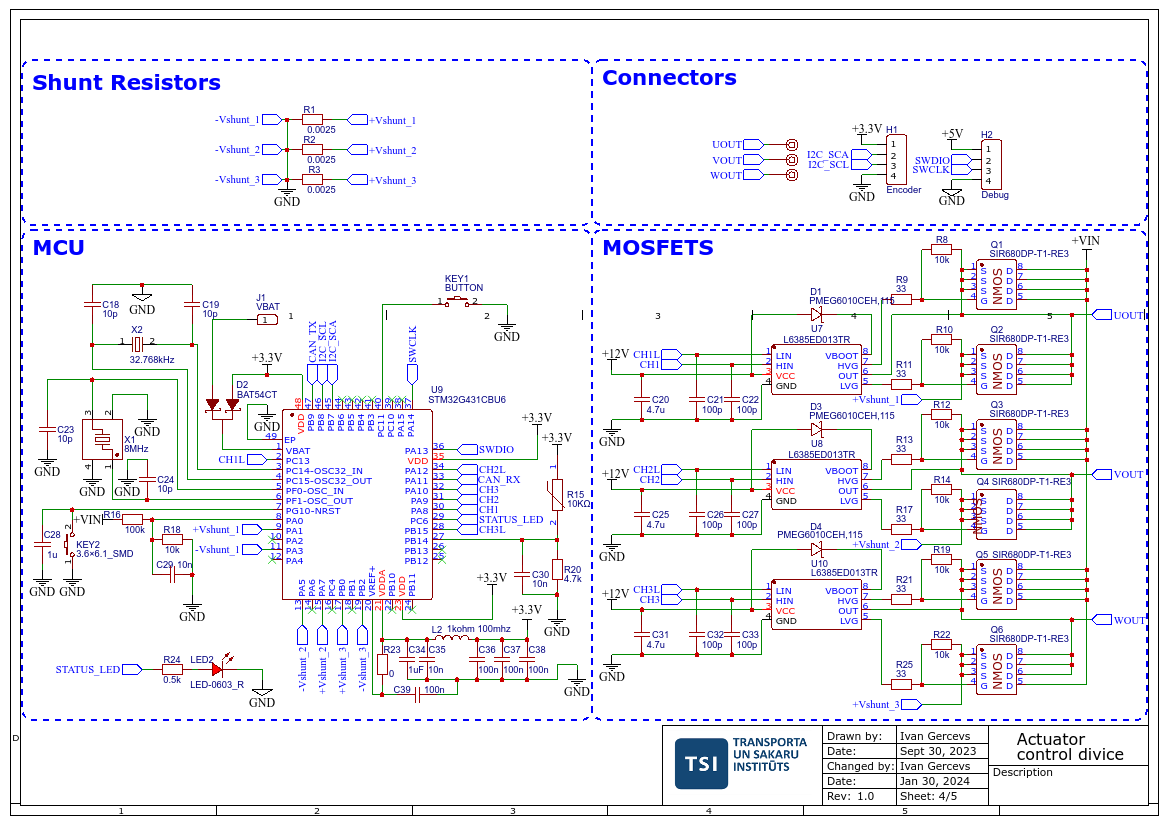
\includegraphics[width=0.85\paperheight]{Src/images/ACD.png}
	\end{adjustbox}
\end{figure}

Драйвера инвертора U7, U8, U10 подключены к выходу таймера TIM1, которые располагаются на линиях порта A и С, для подавления высокочастотных наводок, каждому из входов подключены емкости C21, C22, C26, C27, C32, C33 номиналом 100 пикофарад. Конденсаторы C20, C25, C31 на линии питания установлены, для предотвращения резкого падения напряжений при открытии внутренних силовых транзисторов.  Диоды D1, D3, D4 образуют схему начальной нагрузки, необходимы для обеспечения питания высоковольтной секции драйвера. Драйверы управляют силовыми транзисторами от Q1 - Q6, полумостовой драйвер управляет транзисторами верхней и нижнего уровня для каждой фазы мотора. Транзисторы подключены через низкоомные резисторы R9, R11, R13, R17, R21, R25 для исключения звона (parasitic oscillation) и резисторами R8, R10, R12, R14, R19, R22, резисторы подтягивают затвор к истоку, для избежания паразитных открытий транзисторов.

Для обеспечения связи по шине данных, линии МК PB9 и PA11 подключены к передатчику CAN ШИНЫ U4, принципиальная схема \ref{PPACD}. Передатчик не нуждается в дежурном режиме, поэтому вывод STB (восьмой вывод микросхемы) подключен к земле, передатчик работает с момента включения. Между линиями CANH и CANL предусмотрено включение терминального резистора R7, через перемычку H3. Для удобства монтажа устройств исполнительного управления коннекторы JP2 и JP1 образуют параллельное включение двух разъемов позволяет производить подключений устройств без создания дополнительных соединений на проводах. По такому же принципу подключены силовые разъёмы питания CN1 и CN2.

В данном устройстве реализовано несколько вариантов преобразования напряжений и тока. Основным преобразователем является микросхема DC-DC преобразователя AP64502QSP, которая подключена по стандартной схеме из даташита, принципиальная схема \ref{PPACD}.

Микросхема преобразует входное напряжение в напряжение 12В, которое необходимое для питания драйверов силовых транзисторов. Для обеспечения преобразования напряжения необходимо было рассчитать делитель обратной связи на вход линии FB (Feedback), который вычисляется (\ref{R4}):
\begin{ceqn}
	\begin{align} \label{R4}
		R4=R6\cdot(\frac{V_{out}}{0.8V}-1)
	\end{align}
\end{ceqn}
где R2=10 kOhm, для данного варианты значения получились R1=140 kOhm. Конденсатор С6 на линии SS DC-DC преобразователя является задающим времени мягкого старта. Был выбран стандартный вариант 10nF, чему примерно равен времен мягкого старта - 4 ms. 

\begin{figure}[H]
	\begin{adjustbox}{addcode={\begin{minipage}{\width}}{\caption{
							Принципиальная схема элементов питания и шины данных  системы исполнительного управления
						} \label{PPACD}
					\end{minipage}},rotate=90,center}
		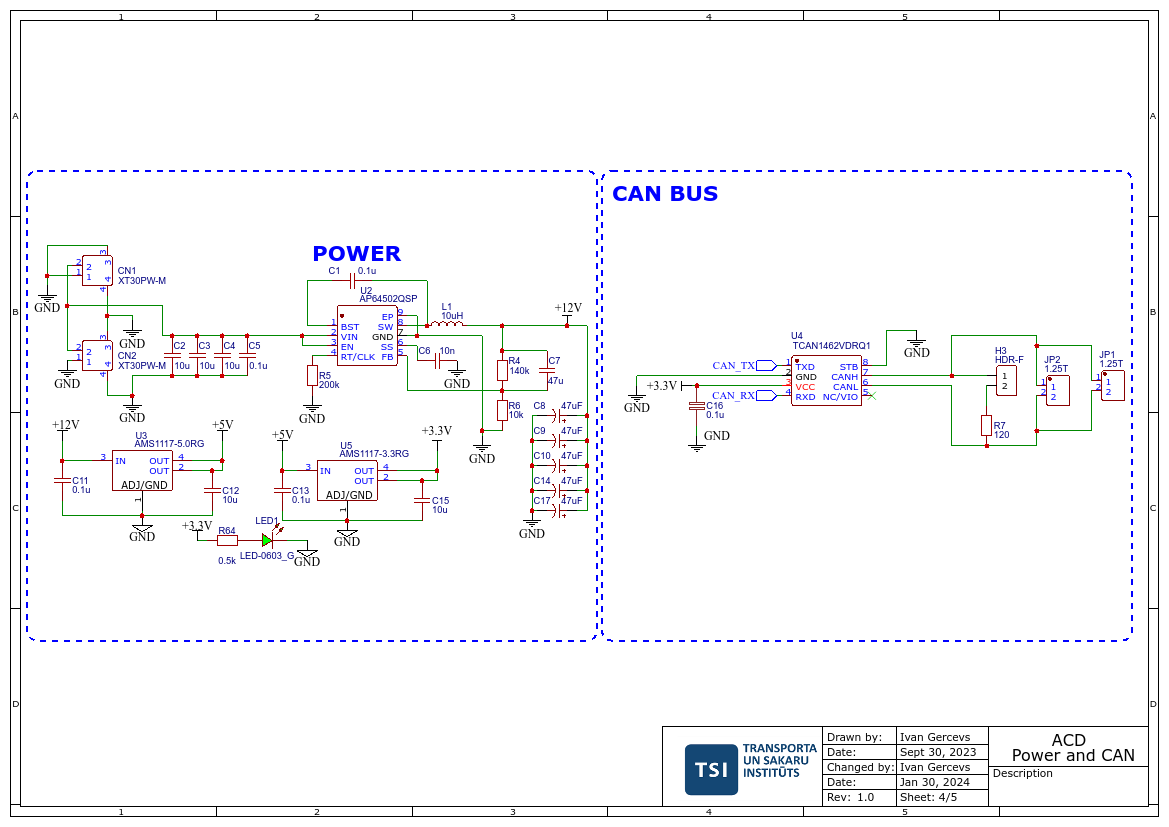
\includegraphics[width=0.85\paperheight]{Src/images/ACD POO.png}
	\end{adjustbox}
\end{figure}

Индуктивность катушки рассчитывается для данного преобразователя по формуле (\ref{L}), где Delta $I_{l}$ при данном подключении рассчитывается по формуле (\ref{Il}):
\begin{ceqn}
	\begin{align} \label{L}
		L = \frac{V_{out}\cdot(V_{in}-V{out})}{V_{in}\cdot\Delta  I_l\cdot f_{sw}}
	\end{align}
\end{ceqn}

\begin{ceqn}
	\begin{align} \label{Il}
		\Delta I_l = 0.5 \cdot 5A
	\end{align}
\end{ceqn}

Микросхема имеет плавную регулировку частоты от 100kHz до 2.2MHz, частота задается резистором R5, частота рассчитывается по формуле (R5):
\begin{ceqn}
	\begin{align} \label{R5}
		R5 = \frac{100000}{f_{sw}[kHz]}
	\end{align}
\end{ceqn}

Для варианта преобразования выбран самый близкий по параметрам индуктивность L = 10 μH. В стандартную схему преобразователя внесен дополнительный ряд сглаживающих танталовых конденсаторов C8, C9, C10, C14, C17. Танталовые конденсаторы имеет маленькое значения внутреннего сопротивления (ESR), который влияет на выходные пульсации (\ref{Vr}):

\begin{ceqn}
	\begin{align} \label{Vr}
		V_{outRipple} = \Delta I_l \cdot (ESR + \frac{1}{8\cdot f_{sw} \cdot C_{cout}})
	\end{align}
\end{ceqn}

Суммарная емкость конденсаторов $5 \times  47\mu F$.

Для преобразования напряжения для микроконтроллеров используются линейные преобразователи напряжения U3 и U5, линейные преобразователи подключены к линии питания 12В для уменьшения   нагрева самих преобразователей, путем уменьшения падения напряжения на них.

Измерение крутящего момента производится за счет измерения тока электродвигателя. Измеряется падения напряжения на шунтах, шунты R1, R2 и R3 имеют очень малое сопротивление, во избежания влияния передаваемое напряжения и излишнего  нагрева. Выводы шунтов подключены ко входам микроконтроллера. После конфигурации микроконтроллера, с линий входа шунтов подключаются ко внутренним операционным усилителям и используются в дальнейших преобразования.

 
\subsection{ Принципиальная схема устройства тактического управления}
Принципиальная схема системы тактического управления устройства мини робота манипулятора представлена на рисунке \ref{PPTCD}.

\begin{figure}[H]
	\begin{adjustbox}{addcode={\begin{minipage}{\width}}{\caption{
							Принципиальная схема системы тактического управления миниробота манипулятора
						} \label{PPTCD}
					\end{minipage}},rotate=90,center}
		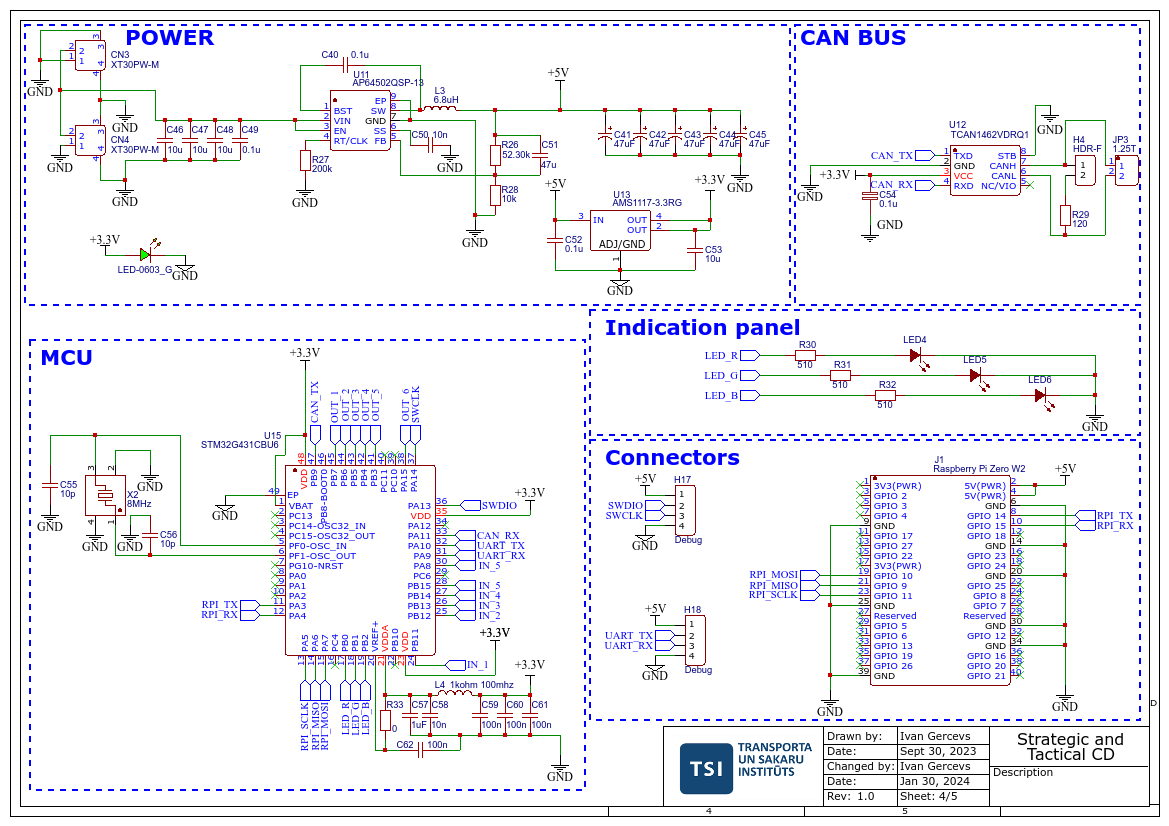
\includegraphics[width=0.85\paperheight]{Src/images/TCD.png}
	\end{adjustbox}
\end{figure}

\begin{figure}[H]
	\begin{adjustbox}{addcode={\begin{minipage}{\width}}{\caption{
							Принципиальная схема входов выводов для системы  управления миниробота манипулятора
						} \label{DI_DOTCD}
					\end{minipage}},rotate=90,center}
		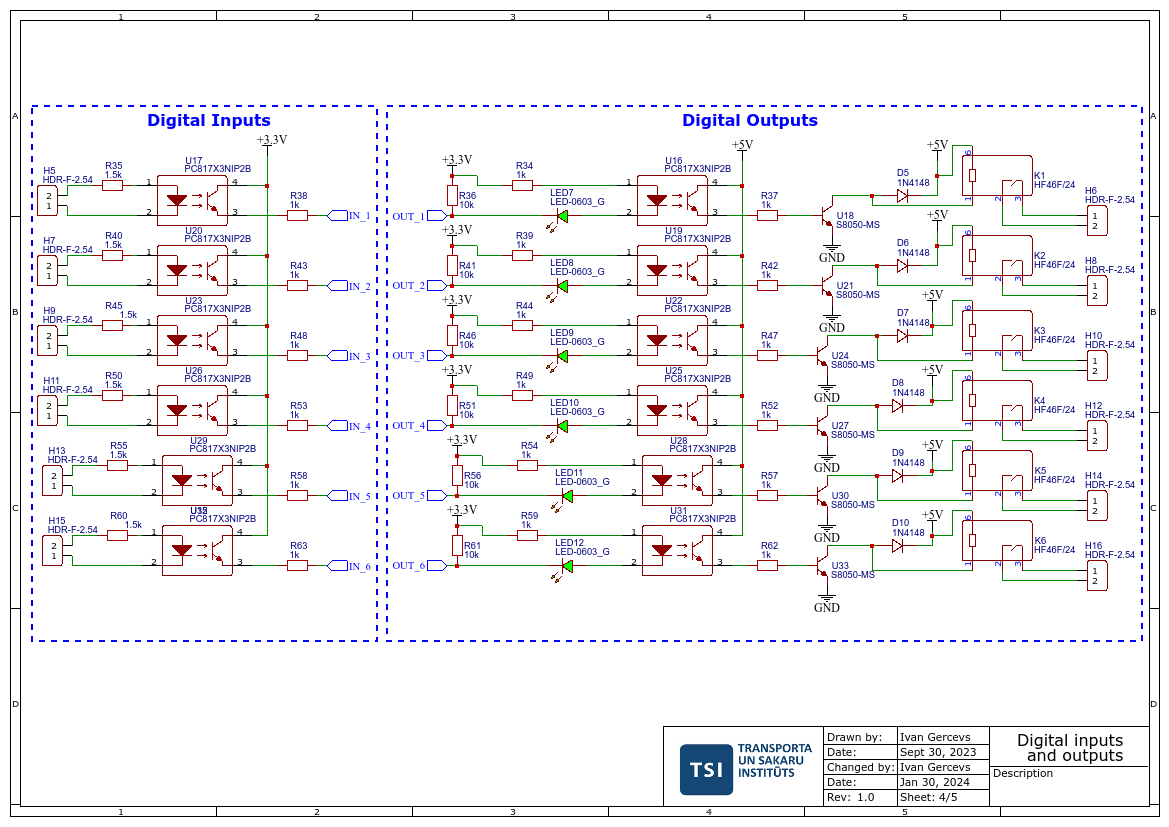
\includegraphics[width=0.85\paperheight]{Src/images/Di_DO.png}
	\end{adjustbox}
\end{figure}

Микроконтроллер U15 является устройством тактического управления и собран по стандартной схеме, как на рисунке \ref{PACD}.  Устройство стратегического управления подключается через разъём J1 и используют два варианта интерфейса SPI и UART. Остальные выводы разъёма J1 не используются, так как к ним могут подключаться различные платы расширения для «Raspberry PI ZERO 2», который расширяют функционал одноплатного миникомпьтера.

Панель индикации состоит из трех светодиодов 3 цветов LED4, LED5, LED6 и подключены ко входу МК. Остальные свободные входы и выходы микроконтроллера разделены для управления внешних сигналы входов (6 штук) и выходов (6 штук) и подключены по стандартной схеме из даташита. 

Входы и выходы изолированы при помощи оптопар, показаны на рисунке \ref{DI_DOTCD}, выходные сигналы коммутируются при помощи реле K1, K2, K3, K4, K5, K6, сигналы с оптопар U16, U19, U22, U25, U28, U31 усиливаются транзисторами U18, U21, U24, U27, U30, U30. Резистор в цепи базы необходим для ограничения тока поступающего на базу транзистора. Диоды D5, D6, D7, D8, D9, D10 необходимы для шунтирования выводов катушки реле в момент отключения питания. В момент выключения, на выводах катушек образуется импульс ЭДС (электродвижущая сила самоиндукции катушки), и этот импульс может достигать десятки Вольт и может привести к выходу из строя транзисторов U18, U21, U24, U27, U30, U30, которые не рассчитан на такое напряжение. 

Входные цифровые сигналы изолируются с помощью U17, U20, U23, U26, U29, U32.  Подразумеваются логическая «1» соответствует 24В напряжения. Для обеспечения включения оптопары произведен расчет резисторов R35, R40, R45, R50, R60, с условием, ток на оптодиод внутри оптопары должен соответствовать 20 mA, при напряжении 1.2 Вольта, допустимое максимальное напряжение 30 Вольт, приближенное значение сопротивления резистора, выбрано из ряда номинала сопротивлений E24 и соответствует 1.5 kOhm. 